\chapter{催化}\label{ch:g12:catalysis}

一瓶过氧化氢溶液在浴室柜中放置
数月而不变。倒在擦伤的膝盖上，它立即起泡：
血液中的某种物质能使它在数秒内分解为水和
氧气。这种物质并不被消耗，也不出现在
反应方程式中。它是一种\omterm{def:g12:catalysis:catalyst}{催化剂}。\omterm{def:g12:catalysis:catalyst}{催化剂}使
大部分化学工业成为可能、净化汽车尾气，并
推动生命中的每一个反应。

\begin{recall}
反应速率，以及改变反应速率的\omterm{def:g12:reaction-rates:kinetic-factor}{动力学因素}
（见\cref{ch:g12:reaction-rates}）。\omterm{def:g12:curly-arrows:mechanism}{反应机理}是由一系列
\omterm{def:g12:curly-arrows:mechanism}{基元反应}组成，并经过\omterm{def:g12:curly-arrows:mechanism}{反应中间体}（见\cref{ch:g12:curly-arrows}）。
\end{recall}

\section{什么是催化剂}

\begin{definition}[催化剂，催化]\label{def:g12:catalysis:catalyst}
称\emph{催化剂}\index{催化剂}为一种能使反应加快的物种，
自身不被消耗：它参与\omterm{def:g12:curly-arrows:mechanism}{反应机理}，最后
原样复原，且不出现在总反应方程式中。
借助催化剂使反应加快的过程称为
\emph{催化}\index{催化}。
\end{definition}

\begin{proposition}[催化剂改变路径，而不改变终点]\label{prop:g12:catalysis:path}
\omterm{def:g12:catalysis:catalyst}{催化剂}开辟了另一条机理，其能垒
低于未\omterm{def:g12:catalysis:catalyst}{催化}反应的能垒，从而使更多的粒子间
碰撞得以生效。它不改变生成物，也不改变
最终达到的状态，只是使其更快到达。
\end{proposition}

\begin{proof}
在本阶段不加证明地承认：能量曲线在本科一年级分册中研究。\omterm{def:g10:reaction-progress-table:system}{最终
状态}不变，源于\omterm{def:g12:catalysis:catalyst}{催化剂}被原样复原：
总反应中的\omterm{def:g7:chemical-reactions:reactant}{反应物}与生成物保持不变。
\end{proof}

\begin{omfigure}
\begin{minipage}{0.49\linewidth}
\begin{tikzpicture}
\begin{axis}[width=\linewidth, height=5.4cm, xmin=0, xmax=1, ymin=-60,
    ymax=110, xtick=\empty, ytick=\empty, axis lines*=left,
    xlabel={反应进程}, ylabel={能量},
    label style={font=\small}, legend style={font=\scriptsize,
    at={(0.02,0.99)}, anchor=north west, draw=none}, legend cell align=left]
  \addplot[very thick, omDef] table[x=s, y=Eu] {figdata/out/grade-12-catalysis-a.dat};
  \addplot[very thick, omProp] table[x=s, y=Ec] {figdata/out/grade-12-catalysis-a.dat};
  \legend{无催化剂, 有催化剂}
  \node[font=\scriptsize, anchor=north west] at (axis cs:0.02,-4) {反应物};
  \node[font=\scriptsize, anchor=south east] at (axis cs:0.99,-36) {生成物};
\end{axis}
\end{tikzpicture}
\end{minipage}\hfill
\begin{minipage}{0.49\linewidth}
\begin{tikzpicture}
\begin{axis}[width=\linewidth, height=5.4cm, xmin=0, xmax=60, ymin=0,
    ymax=80, xlabel={$t$ (\si{min})}, ylabel={\ce{O2} 放出量 (\si{mL})},
    axis lines*=left, ymajorgrids, grid style={gray!20},
    tick label style={font=\scriptsize}, label style={font=\small},
    legend style={font=\scriptsize, at={(0.98,0.03)}, anchor=south east,
    draw=none}, legend cell align=left]
  \addplot[very thick, omDef] table[x=t, y=Vu] {figdata/out/grade-12-catalysis-b.dat};
  \addplot[very thick, omProp] table[x=t, y=Vc] {figdata/out/grade-12-catalysis-b.dat};
  \legend{无催化剂, 有催化剂}
\end{axis}
\end{tikzpicture}
\end{minipage}

{\small 左图：沿反应进程的能量变化；\omterm{def:g12:catalysis:catalyst}{催化}途径经过一个中间体，
经历两个较低的能垒。右图：过氧化氢溶液放出的氧气；\omterm{def:g12:catalysis:catalyst}{催化剂}
加快了反应，但最终体积相同。
（示意曲线）}
\end{omfigure}

\section{均相催化}

\begin{definition}[均相催化与多相催化]\label{def:g12:catalysis:homogeneous}
\omterm{def:g12:catalysis:catalyst}{催化剂}与\omterm{def:g7:chemical-reactions:reactant}{反应物}处于同一相时，此类\omterm{def:g12:catalysis:catalyst}{催化}称为\emph{均相催化}\index{均相催化}
（例如与\omterm{def:g7:chemical-reactions:reactant}{反应物}一同\omterm{def:g2:mixing-and-dissolving:dissolve}{溶解}），
\omterm{def:g12:catalysis:catalyst}{催化剂}处于另一相时，称为\emph{多相催化}\index{多相催化}，
通常是固体，\omterm{def:g7:chemical-reactions:reactant}{反应物}从气体或液体中
到达其表面。
\end{definition}

\begin{example}[碘离子与过氧化氢]\label{ex:g12:catalysis:iodide}
过氧化氢自行分解得非常缓慢：
\ce{2H2O2 -> 2H2O + O2}。在其中\omterm{def:g2:mixing-and-dissolving:dissolve}{溶解}少量碘化钾后，
溶液立即起泡。碘\omterm{def:g9:ions:ion}{离子}分两步开辟一条途径：
\[
  \ce{H2O2 + I- -> H2O + IO-}, \qquad
  \ce{H2O2 + IO- -> H2O + O2 + I-} .
\]
两步相加得 \ce{2H2O2 -> 2H2O + O2}：
其中碘\omterm{def:g9:ions:ion}{离子}在第一步中被消耗、第二步中又生成，是\omterm{def:g12:catalysis:catalyst}{催化剂}；
\ce{IO-} 是中间体。
\end{example}


\begin{example}[三价铁离子]\label{ex:g12:catalysis:iron}
三价铁\omterm{def:g9:ions:ion}{离子}也能\omterm{def:g12:catalysis:catalyst}{催化}该分解，通过电对
\ce{Fe^{3+}}/\ce{Fe^{2+}}（见\cref{ch:g11:redox}）：三价铁先氧化
过氧化氢，\ce{2Fe^{3+} + H2O2 -> 2Fe^{2+} + O2 + 2H+}，然后
生成的二价铁\omterm{def:g9:ions:ion}{离子}被更多的过氧化氢重新氧化，
\ce{2Fe^{2+} + H2O2 + 2H+ -> 2Fe^{3+} + 2H2O}。溶液原本的浅橙色
在放出气体时变为偏绿色，随后
待过氧化氢耗尽后又恢复，这表明\omterm{def:g12:catalysis:catalyst}{催化剂}参与了反应
并被再生。
\end{example}

\section{多相催化}

许多工业\omterm{def:g12:catalysis:catalyst}{催化剂}是固体，如铂、钯、
镍或铁等\omterm{def:g9:periodic-table-first-look:metal}{金属}，或氧化物。反应发生在它们的表面上，
分三个阶段进行：\omterm{def:g7:chemical-reactions:reactant}{反应物}\omterm{def:g7:atoms-and-molecules:molecule}{分子}先被固定在表面上
（吸附），其化学键在此被削弱；随后在表面上发生反应；
生成物离开表面，表面重新空出，可容纳新的\omterm{def:g7:atoms-and-molecules:molecule}{分子}。因此，
\omterm{def:g12:catalysis:catalyst}{催化剂}通常制成尽可能大的表面积：细粉末，或
涂覆在多孔载体上的薄层。

\begin{omfigure}
\begin{tikzpicture}[font=\small]
  \foreach \x in {0,4.2,8.4} {
    \fill[black!25] (\x,0) rectangle (\x+3.4,0.35);
    \foreach \i in {0,1,2,3,4,5,6,7} \shade[ball color=black!35] (\x+0.21+\i*0.425,0.35) circle (0.2);
  }
  % 1. adsorption
  \node[aH, minimum size=3.2mm] at (0.9,0.75) {};
  \node[aH, minimum size=3.2mm] at (1.3,0.75) {};
  \node[aH, minimum size=3.2mm] (h1) at (2.2,1.8) {};
  \node[aH, minimum size=3.2mm] (h2) at (2.6,1.8) {};
  \draw[bond, line width=1.2pt] (h1.east) -- (h2.west);
  \draw[->, omProp, thick] (2.4,1.55) -- (2.0,1.0);
  \node[anchor=north, align=center] at (1.7,-0.1) {1. 吸附：\\ \ce{H-H} 键断裂};
  % 2. reaction on the surface
  \node[aC] (c1) at (5.5,1.05) {}; \node[aC] (c2) at (6.2,1.05) {};
  \draw[bond, line width=1.4pt] (c1) -- (c2);
  \node[aH, minimum size=3.2mm] at (5.3,0.75) {};
  \node[aH, minimum size=3.2mm] at (6.6,0.75) {};
  \node[anchor=north, align=center] at (5.9,-0.1) {2. H 原子加到 \\ 吸附的分子上};
  % 3. desorption
  \node[aC] (c3) at (9.6,1.8) {}; \node[aC] (c4) at (10.3,1.8) {};
  \draw[bond, line width=1.4pt] (c3) -- (c4);
  \foreach \a/\c in {150/c3,210/c3,90/c3,30/c4,-30/c4,90/c4}
    \node[aH, minimum size=2.8mm] at ($(\c)+(\a:0.42)$) {};
  \draw[->, omProp, thick] (11.0,1.2) -- (11.0,2.2);
  \node[anchor=north, align=center] at (10.1,-0.1) {3. 生成物 \\ 离开表面};
\end{tikzpicture}

{\small 氢气在\omterm{def:g9:periodic-table-first-look:metal}{金属}表面与乙烯加成：吸附，
反应、脱附。\omterm{def:g9:periodic-table-first-look:metal}{金属}本身未发生变化。}
\end{omfigure}

\begin{example}[催化转化器]\label{ex:g12:catalysis:converter}
汽油机的尾气中含有一氧化碳和一氧化氮，
两者均有毒，并含有未\omterm{def:g4:what-a-fire-needs:burning}{燃烧}的\omterm{def:g4:what-a-fire-needs:fuel}{燃料}。在\omterm{def:g12:catalysis:catalyst}{催化}转化器中，
陶瓷蜂窝体涂有铂和铑，气体在
\omterm{def:g9:periodic-table-first-look:metal}{金属}表面上发生反应：
\[
  \ce{2CO + 2NO -> 2CO2 + N2} ,
\]
碳氢化合物\omterm{def:g4:what-a-fire-needs:burning}{燃烧}生成二氧化碳和水。气体
在极短的时间内通过转化器，
无\omterm{def:g12:catalysis:catalyst}{催化剂}时反应来不及发生。
\end{example}

\begin{omfigure}
\begin{tikzpicture}[font=\small]
  \fill[black!12, draw=black!60, rounded corners=6pt] (0,0) rectangle (6,2.4);
  \foreach \x in {0.3,0.6,0.9,1.2,1.5,1.8,2.1,2.4,2.7,3.0,3.3,3.6,3.9,4.2,4.5,4.8,5.1,5.4,5.7} \draw[black!35] (\x,0.2) -- (\x,2.2);
  \foreach \y in {0.5,0.9,1.3,1.7,2.1} \draw[black!35] (0.2,\y) -- (5.8,\y);
  \fill[black!40] (-1.4,0.9) rectangle (0,1.5);
  \fill[black!40] (6,0.9) rectangle (7.4,1.5);
  \draw[->, very thick, omThm] (-2.6,1.2) -- (-1.5,1.2);
  \node[anchor=east, align=right, omThm] at (-2.7,1.2) {\ce{CO}、\ce{NO}、\\ 碳氢化合物};
  \draw[->, very thick, omMeth] (7.5,1.2) -- (8.6,1.2);
  \node[anchor=west, align=left, omMeth] at (8.7,1.2) {\ce{CO2}, \ce{N2},\\ \ce{H2O}};
  \node[align=center, fill=white, inner sep=2pt] at (3,1.2) {陶瓷蜂窝体 \\ 涂有 Pt 和 Rh};
\end{tikzpicture}

{\small 纵向剖开的\omterm{def:g12:catalysis:catalyst}{催化}转化器：数千条细小通道
为尾气提供巨大的\omterm{def:g9:periodic-table-first-look:metal}{金属}涂层表面。}
\end{omfigure}

\begin{omfigure}
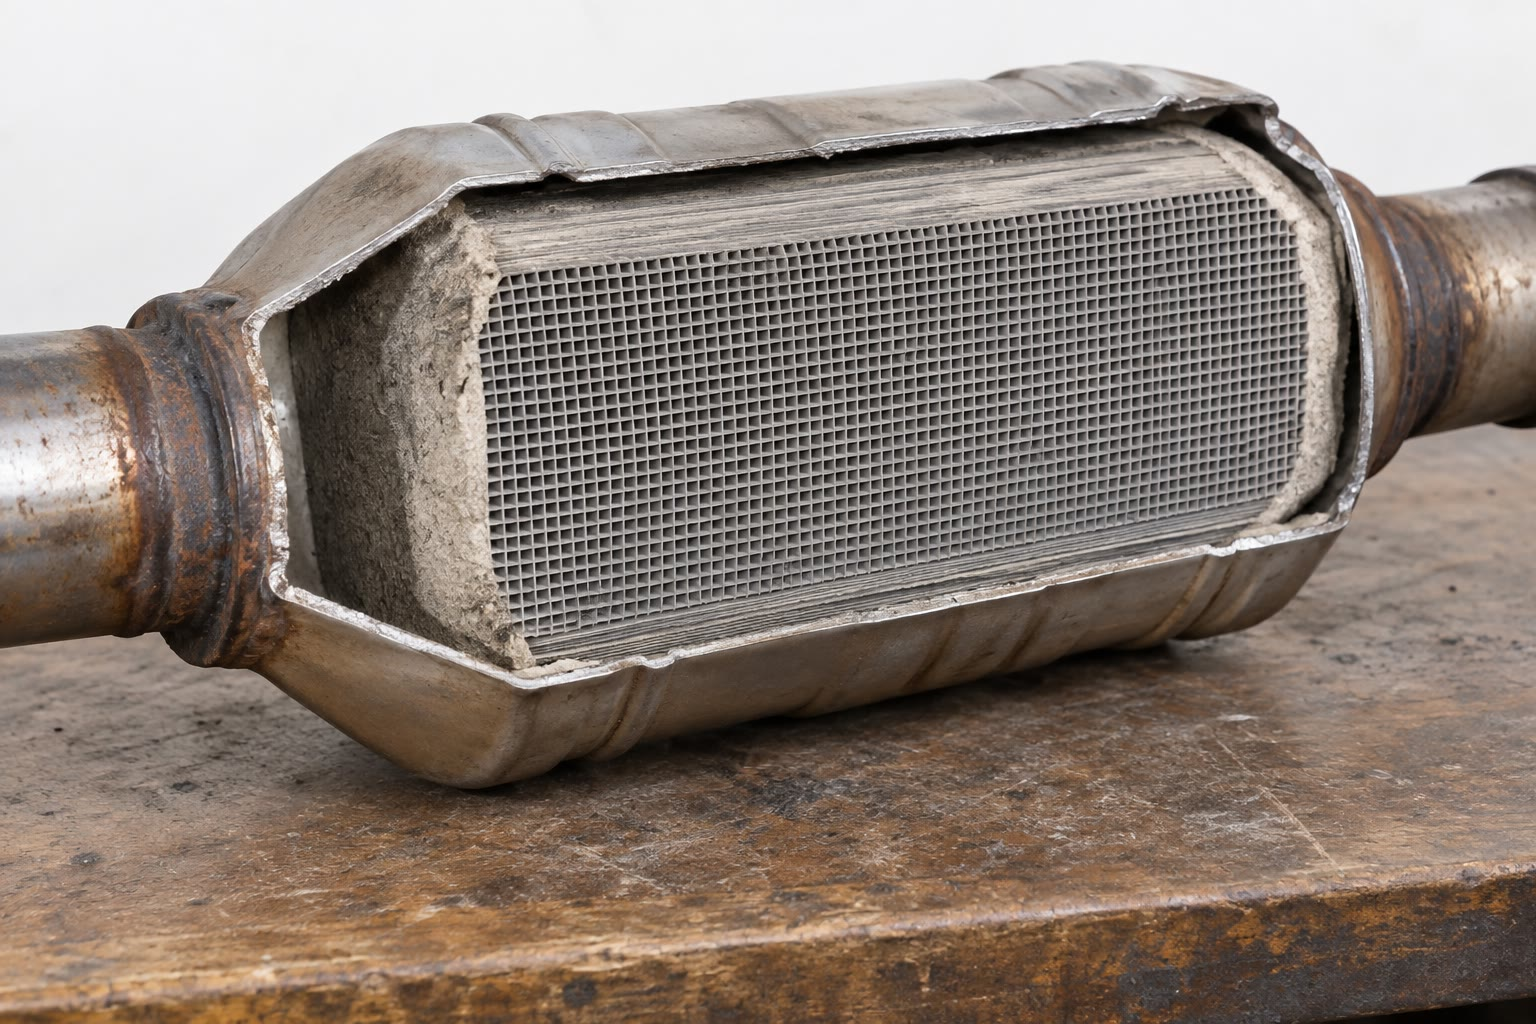
\includegraphics[width=0.45\linewidth]{images/book1/ai/g12-catalytic-converter.jpg}

{\small 剖开的\omterm{def:g12:catalysis:catalyst}{催化}转化器：蜂窝芯体。}
\end{omfigure}

\begin{history}[哈伯、博施与氨]
% ledger: haber:T, haber:p, nh3:world-2024
二十世纪初，化学家哈伯
找到了将\omterm{def:g4:air-a-mixture-of-gases:air}{空气}中的氮与氢结合的方法，
\ce{N2 + 3H2 -> 2NH3}，在铁基\omterm{def:g12:catalysis:catalyst}{催化剂}上实现；工程师卡尔·
博施将其变为工业过程，至今仍在 400
至 \qty{500}{\celsius}、150 至 \qty{250}{atm} 下运行。2024 年，全球
生产的氨约含氮 1.5 亿吨，其中大部分用于化肥：
人们所吃食物中的氮，很大一部分
都经过了这类\omterm{def:g12:catalysis:catalyst}{催化剂}。
\end{history}

\section{酶}

\begin{definition}[酶]\label{def:g12:catalysis:enzyme}
称\emph{酶}\index{酶}为由生物体\omterm{def:g10:synthesis-yield:synthesis}{合成}的一类蛋白质，
能\omterm{def:g12:catalysis:catalyst}{催化}其体内的某一种反应。酶的效率很高，
专一性也很强：每种酶只作用于少数几种\omterm{def:g7:atoms-and-molecules:molecule}{分子}，且
仅在较窄的温度和酸碱度范围内效果最好。
\end{definition}

\begin{example}[过氧化氢酶]\label{ex:g12:catalysis:catalase}
过氧化氢在细胞中作为副产物生成，对细胞有害。
过氧化氢酶存在于血液、肝脏及许多植物组织中，
能以极快的速度将其分解为水和氧气：这正是
擦伤的膝盖上或生土豆片上出现泡沫的原因。煮熟的土豆
不产生泡沫：加热破坏了酶的结构。
\end{example}

\begin{omfigure}
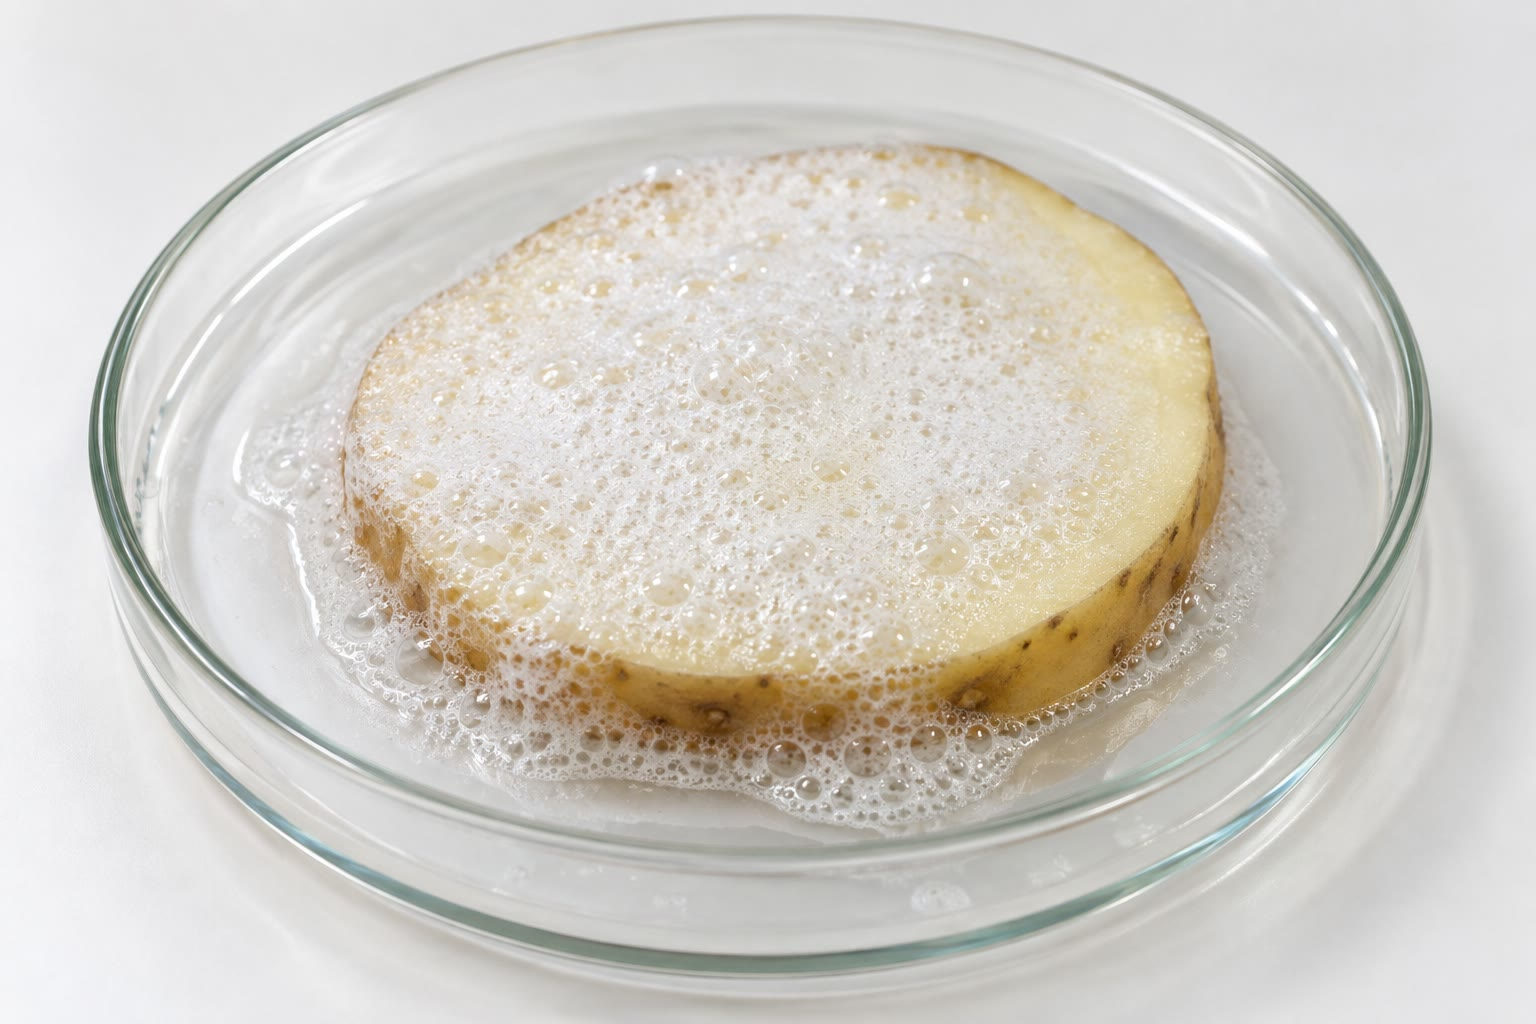
\includegraphics[width=0.45\linewidth]{images/book1/ai/g12-potato-peroxide.jpg}

{\small 生土豆片上的过氧化氢：过氧化氢酶正在发挥作用。}
\end{omfigure}

\section{选择性}

\begin{definition}[选择性催化剂]\label{def:g12:catalysis:selective}
当同一\omterm{def:g7:chemical-reactions:reactant}{反应物}可以发生几个反应时，一种\emph{选择性
催化剂}\index{选择性催化剂}能使其中某一反应的速率远大于其他反应，
从而决定生成哪些生成物。
\end{definition}

\begin{example}[乙醇的两种去向]\label{ex:g12:catalysis:ethanol}
热的乙醇蒸气通过氧化铝时失去水，生成乙烯，
\ce{C2H5OH -> C2H4 + H2O}（\omterm{def:g12:curly-arrows:categories}{消除}）；通过热铜时，它
失去氢，生成乙醛，\ce{C2H5OH -> CH3CHO + H2}。
同一\omterm{def:g7:chemical-reactions:reactant}{反应物}，两种\omterm{def:g12:catalysis:catalyst}{催化剂}，两种生成物。
\end{example}

\begin{remark}[工业与生命都依靠催化剂]\label{rem:g12:catalysis:everywhere}
化学工业的大多数产品，从\omterm{def:g4:what-a-fire-needs:fuel}{燃料}到\omterm{def:g8:plastics:plastic}{塑料}和
化肥等，大多借助\omterm{def:g12:catalysis:catalyst}{催化剂}制成；找到活性更高
或选择性更好的\omterm{def:g12:catalysis:catalyst}{催化剂}，可节约能量、减少废物。活细胞内的每一个反应
都由酶\omterm{def:g12:catalysis:catalyst}{催化}。
\end{remark}

\begin{safety}{\ghs[0.82cm]{GHS03}\ghs[0.82cm]{GHS05}\ghs[0.82cm]{GHS07}}
% ledger: ghs:H2O2
浓过氧化氢是一种强\omterm{def:g11:redox:oxidant}{氧化剂}，能助燃，
会灼伤皮肤和眼睛，误食有害。实验室中的稀
溶液使用时仍须佩戴护目镜和手套；
分解会放出氧气，因此绝不可在密闭容器中进行。
\end{safety}

\section{练习}


\begin{exercise}[$\star$]\label{exo:g12:catalysis:1}
在碘\omterm{def:g9:ions:ion}{离子}\omterm{def:g12:catalysis:catalyst}{催化}的过氧化氢分解反应中，哪些
物种是\omterm{def:g7:chemical-reactions:reactant}{反应物}，哪些是生成物，哪一种是\omterm{def:g12:catalysis:catalyst}{催化剂}，
哪一种是中间体？
\end{exercise}

\begin{exercise}[$\star$]\label{exo:g12:catalysis:2}
判断下列各例属于\omterm{def:g12:catalysis:homogeneous}{均相催化}还是\omterm{def:g12:catalysis:homogeneous}{多相催化}：过氧化氢溶液中的碘\omterm{def:g9:ions:ion}{离子}；
\omterm{def:g12:catalysis:catalyst}{催化}转换器中的铂；\omterm{def:g10:synthesis-yield:synthesis}{合成}氨工业中的
铁；过氧化氢溶液中的铁(III)\omterm{def:g9:ions:ion}{离子}？
\end{exercise}

\begin{exercise}[$\star$]\label{exo:g12:catalysis:3}
在能量曲线图上，哪条路径的能垒更高？两条路径的
始态与终态能量是否相同？这对
生成物意味着什么？
\end{exercise}

\begin{exercise}[$\star$]\label{exo:g12:catalysis:4}
为什么\omterm{def:g12:catalysis:catalyst}{催化剂}不出现在反应的总方程式中？
\end{exercise}

\begin{exercise}[$\star$]\label{exo:g12:catalysis:5}
为什么工业上的固体\omterm{def:g12:catalysis:catalyst}{催化剂}要制成细粉，或
以薄涂层形式附着于多孔载体上？
\end{exercise}

\begin{exercise}[$\star\star$]\label{exo:g12:catalysis:6}
将铁(III)\omterm{def:g12:catalysis:catalyst}{催化}过氧化氢分解的两个步骤
相加，并说明铁\omterm{def:g9:ions:ion}{离子}与氢\omterm{def:g9:ions:ion}{离子}相互抵消。
\end{exercise}

\begin{exercise}[$\star\star$]\label{exo:g12:catalysis:7}
读取所放出氧气的曲线。每次实验放出最终体积
一半所需的时间各是多少？\omterm{def:g12:catalysis:catalyst}{催化剂}使它
缩短了多少倍？
\end{exercise}

\begin{exercise}[$\star\star$]\label{exo:g12:catalysis:8}
装有\omterm{def:g12:catalysis:catalyst}{催化}转换器的汽车不使用含铅汽油：铅
会沉积在铂上并留在那里。试解释这为何会使
转换器失效，尽管铂在正常反应中并不会被消耗。
\end{exercise}

\begin{exercise}[$\star\star$]\label{exo:g12:catalysis:9}
某同学测量了生土豆片在过氧化氢溶液中产生的泡沫，
在 10、25、37、60 和 \qty{80}{\celsius} 下，泡沫量
先增至约 \qty{37}{\celsius} 左右，随后下降，
并在 \qty{80}{\celsius} 时几乎消失。试解释曲线的两个部分。
\end{exercise}

\begin{exercise}[$\star\star$]\label{exo:g12:catalysis:10}
写出\omterm{def:g12:catalysis:catalyst}{催化}转换器中一氧化碳与
一氧化氮反应的方程式，并检验其是否配平。
为什么这两种污染物能同时被除去？
\end{exercise}

\begin{exercise}[$\star\star$]\label{exo:g12:catalysis:11}
\qty{10.0}{mL} 过氧化氢溶液完全分解可放出 \qty{72}{mL}
\qty{20}{\celsius} 下的氧气。计算
氧气的\omterm{def:g10:the-mole:amount}{物质的量}（$V_m = \qty{24.1}{L/mol}$），再求该溶液中过氧化氢的\omterm{def:g10:concentration-and-dilution:molar-concentration}{物质的量浓度}。
在过氧化氢溶液中的\omterm{def:g10:concentration-and-dilution:molar-concentration}{物质的量浓度}。
\end{exercise}

\begin{exercise}[$\star\star\star$]\label{exo:g12:catalysis:12}
乙醇蒸气通过氧化铝得到乙烯；通过铜则得到
乙醛。写出两个方程式，说明第一个反应的类型，并
解释什么是\omterm{def:g12:catalysis:selective}{选择性催化剂}。
\end{exercise}

\begin{exercise}[$\star\star\star$]\label{exo:g12:catalysis:13}
\omterm{def:g12:catalysis:catalyst}{催化剂}可使反应速率加快十倍。某同学认为它也
能使生成物增加十倍。请利用所放出氧气的曲线
修正这一说法。
\end{exercise}

\begin{exercise}[$\star\star\star$]\label{exo:g12:catalysis:14}
一个过氧化氢酶\omterm{def:g7:atoms-and-molecules:molecule}{分子}每秒大约分解几百万个
过氧化氢\omterm{def:g7:atoms-and-molecules:molecule}{分子}。取每秒 $\num{5e6}$ 个，一个酶\omterm{def:g7:atoms-and-molecules:molecule}{分子}
分解一\omterm{def:g10:the-mole:amount}{摩尔}过氧化氢需要多长时间？
若在一秒内完成这一分解，需要多少个酶\omterm{def:g7:atoms-and-molecules:molecule}{分子}？（
这是关于数量级的计算；速率为练习给定的数据。）
\end{exercise}

\begin{exercise}[$\star\star\star$]\label{exo:g12:catalysis:15}
% ledger: nh3:world-2024
2024 年，全世界约制得 1.5 亿吨以氨形式存在的氮。
这些氮对应多少质量的氨？所结合的氮气的\omterm{def:g10:the-mole:amount}{物质的量}是多少？
\end{exercise}

\section{问题：理发师的过氧化氢}

\begin{problem}[{周末问题——“20 体积”过氧化氢的
浓度是多少？}]
\label{pb:g12:catalysis:1}
% ledger: const:Vm1, ghs:H2O2, aw:H, aw:O
理发师使用以“体积”标注的过氧化氢溶液：一种
“20 体积”溶液是指每 \qty{1}{L} 溶液完全分解时可放出 \qty{20}{L}
的氧气，该气体在
\qty{0}{\celsius} 和标准大气压下测量，此时一\omterm{def:g10:the-mole:amount}{摩尔}气体
的体积为 \qty{22.4}{L}。

\medskip
\noindent\textbf{第一部分——分解反应。}
\begin{enumerate}
  \item 写出过氧化氢分解的方程式。
  \item 该分解反应是否为\omterm{def:g11:redox:reaction}{氧化还原反应}？找出\omterm{def:g11:redox:oxidant}{氧化剂}和\omterm{def:g11:redox:oxidant}{还原剂}
        （过氧化氢两者皆是）。
  \item 反应可以发生，为何一瓶过氧化氢能保存数月
        却不分解？
\end{enumerate}

\medskip
\noindent\textbf{第二部分——“20 体积”的含义。}
\begin{enumerate}[resume]
  \item \qty{1}{L} 该溶液放出的氧气\omterm{def:g10:the-mole:amount}{物质的量}是多少？
  \item 推算 \qty{1}{L} 溶液中过氧化氢的\omterm{def:g10:the-mole:amount}{物质的量}。
  \item 求出\omterm{def:g10:concentration-and-dilution:molar-concentration}{物质的量浓度}。
  \item 计算过氧化氢的\omterm{def:g10:the-mole:molar-mass}{摩尔质量}及
        \omterm{def:g10:concentration-and-dilution:mass-concentration}{质量浓度}。
  \item “10 体积”若用\omterm{def:g10:the-mole:amount}{摩尔}每升表示，其含义如何？
\end{enumerate}

\medskip
\noindent\textbf{第三部分——两种\omterm{def:g12:catalysis:catalyst}{催化剂}。}
\begin{enumerate}[resume]
  \item 向样品中分别加入一滴血液（即过氧化氢酶）和几滴三氯化铁，
        两者各属于何种\omterm{def:g12:catalysis:catalyst}{催化}？
  \item 写出三氯化铁\omterm{def:g12:catalysis:catalyst}{催化}的两个步骤，并检验
        两步之和是否为分解反应。
  \item 利用所放出氧气的曲线，描述有无\omterm{def:g12:catalysis:catalyst}{催化剂}时氧气的
        体积变化情况，以及哪些量
        保持不变。
  \item 三氯化铁\omterm{def:g12:catalysis:catalyst}{催化}的样品，其颜色在反应中为何会变化，
        并在反应结束时复原？
  \item 为何煮过的土豆不会使溶液起泡？
\end{enumerate}

\medskip
\noindent\textbf{第四部分——储存瓶。}
\begin{enumerate}[resume]
  \item 在 \qty{0}{\celsius} 下测量，一个
        \qty{100}{mL} 的瓶子最多能放出多少体积的氧气？
  \item 该体积在 \qty{20}{\celsius} 下是多少？（$V_m =
        \qty{24.1}{L/mol}$）？
  \item 这类瓶子的瓶盖为何必须让气体缓慢逸出？
  \item 一瓶长期储存的过氧化氢经\omterm{def:g11:titration:titration}{滴定}，发现其
        浓度为 \qty{1.50}{mol/L}，这相当于现在多少“体积”？
  \item 过氧化氢已分解的比例是多少？
  \item 给出最终答案：一瓶
        “20 体积”过氧化氢溶液的\omterm{def:g10:concentration-and-dilution:molar-concentration}{物质的量浓度}是多少？
\end{enumerate}
\end{problem}
